\documentclass[a4paper]{dnd5}
\begin{document}
\pagestyle{empty}

\newtoggle{DM}
\toggletrue{DM}
%\togglefalse{DM}

\section*{Orcs and Goblins}

The Orcs are a green skinned race that live in the North Eastern Steppes most often called the Orcish Wastes.  They stand seven foot tall or more and their bodies are packed with thick ropey muscles.  They are both strong and physically robust, they are inured to the bitter cold of the steppes, and they can go a long time without food.  Orcs like to eat meat and they prefer the flesh of elves, humans, halflings and other orcs above all else.  

\vspace{0.4em}
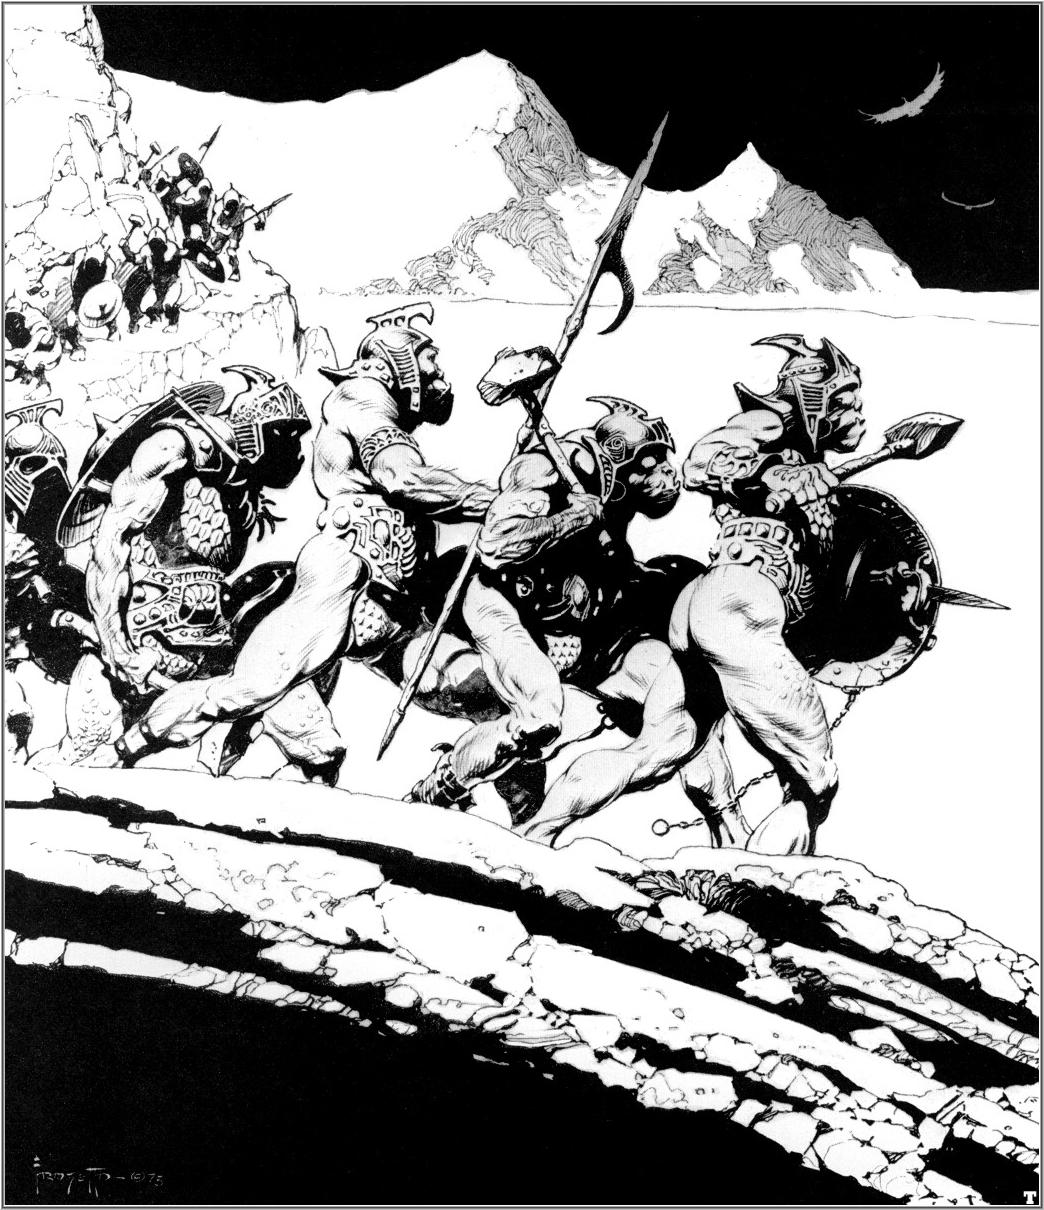
\includegraphics[width=0.45\textwidth]{orcs.jpg}
\vspace{0.4em}

Orcs are quick to anger and may become unthinkingly enraged in a matter of seconds given the right circumstance.  This state is called Graua and can quickly take hold amongst a group of Orcs in what is thought to be a type of mass hysteria.  Gruaa is one of the reasons that Orcs are such a fearsome enemy.  Even the sturdiest city walls can fall to thousands of Orcs who climb the walls unthinking of their own self preservation.  Orcs who exhibit outstanding blood rage are gifted with many females by their chiefs.   Consequently, there is a great deal of competition between Orcs to demonstrate who among them is the most fearless.  It is extremely insulting to Orcs to question their bravery.  It is perhaps not surprising then that the Orcish language has many many terms that describe cowardice such as Ergosh which means one-who-stands-in-line (a reference to those who hang back in the shield wall during a battle), and Gelash (which means Elf-hearted).

They are a cruel and unintelligent race who delight in the suffering of 
others.  Individually, Orcs are untrustworthy.  Their word in a bargain is only good as long as the Orc sees any benefit in the bargain for themselves.  They are quite stupid beings.  Virtues that are prized by Orcs are: blood thirstiness, cruelty and cunning.  Orcs have a large range of epic tales that are told during the long nights usually accompanied by a kind of tabor drum.  Their tales often feature Gorosh the Mighty, Magog, or Harash the Sly.  In these tales Gorosh usually ends up killing the children of his enemies.  Magog is a great hero and leader who shows mercy to his enemies after he has vanquished them and ends up getting his throat cut.  Harash declares some object of his desire, sometimes a female, sometimes treasure, sometime a chieftainship, and he then proceeds to poison or stab quite a number of people and before achieving his goal in an extremely circuitous and humorous manner.  The Orcish oral tradition is quite rich and there are a number of other minor heroes that feature in the less popular tales.

Orcs are tremendously fecund, forming great nomadic tribes that roam the wilderness.  Thankfully the orcs are a fractious race, else their vast numbers would effortlessly wash away the cities of man.  Orcs spend a great deal of their time fighting amongst one another.  The members of Orcish tribes are careful to demonstrate their strength to other tribes at any opportunity, as any tribe that appears weak is quickly exterminated by other orcish tribes. 

Various Orcish tribes practice slavery.  The practice is not widely spread because most Orcs usually kill and eat their slaves after very short periods of time.  Certainly they keep no sick, old or young slaves. Slaves are used for mining, and building projects (walled towns, huts and crude ships to travel on large rivers).  Orcs themselves have little talent for building and most prefer to sleep outside than build.

From time to time human rulers have struck treaties with various Orc tribes. None has held for any length of time.  There is a famous Orcish tale about how Harash joined forces with a Thule King and sacked the city of Yronberg.  After being paid, Harash poisoned the King and his followers and turned on the Thule army slaughtering them all in the night.  It is widely regarded as one of the most amusing tales featuring Harash.

Orcs do trade with humans. They sell hides, the tusks of mammoths, metals they force slaves to dig for, and treasures they have raided from civilized people.  Orcs purchase iron, weapons, barrels, tools and pipeweed.  Periodically the temptation becomes too great for the Orcs and they attack the merchants who they are dealing with.  This usually brings trading in the region to a halt for some time.

Orcs drink a stagnant alcoholic drink they call Borosh that they make by fermenting grass, bark, moss, lichen and whatever else happens to be available.  Drinking borosh can make you blind, which in Orcish society is fatal.  This doesn't seem to stop them however as they drink enormous amounts of the liquid.

Most members of this foul race have very little self-control or patience.  Orc armies never siege a city for more than a few days (while they pillage the surrounding country side, rest up and look for weaknesses in the city's walls).  They almost always assault cities and towns after this time as they grow bored.  Orcs never use siege engines of any kind.  They have the technological ability, but not the temperament, to do so.  Orcs never build anything themselves - the effort required always deemed too great.

Orcs are closely related to Goblins, though they do not acknowledge the fact.  The two are in fact different species.  They are also less closely related to giants and trolls.  All these species share the same guttural language, though there are a large number of different dialects.

Technologically, the orcs are fairly primitive.  Their grasp over iron work is basic at best.  They have a written language but only a small number of Orcs know how to read or write it.  They do not build boats but they will sail in them if they find them or if they have slaves build boats for them, swimming across smaller rivers and travelling around larger ones.  In the north They herd large populations of reindeer for food, and their hides.

Orcs travel in small groups, in warbands containing dozens of warriors, and in tribes which may contain as many as a thousand or more Orcs.  Tribes contain females, and the young, larges packs of herd animals, possibly some slaves and many many fighting orcs.  There are no old Orcs.  Tribes are ruled by an Okash, (a chief).  Periodically a great charismatic leader arises and consolidates a number of Orcish tribes into a great Orcish horde.  These hordes are so large that they cannot sustain themselves by hunting and gathering.  They move through the icey wastes annihilating or absorbing any Orcish tribes they meet.  They sweep down from the north through the lands of man killing and burning.  When they meet one of the large walled cities on the boundaries of civilized nations they either break like a wave on the rocks or wash over the city destroying it.   Thankfully, Orcish hordes tend not to last too long as their leaders are often assassinated or poisoned by internal rivals.  If an Orcish horde fails in its attempts to assault a human city the Orcish leader will always be killed by his subordinates (unless he finds a way to flee).
\end{document}
